\part{Betinget Optimering}

\chapter{Introduksjon til Betinget Optimering}

I dette kapittelet skal vi se på betinget optimering, som er en viktig del av optimeringsteori. Betinget optimering handler om å finne minimum eller maksimum av en funksjon når vi har begrensninger på variablene.

\section{Problemformulering}

Et typisk betinget optimeringsproblem kan skrives på formen:
\begin{align*}
	\min_{x \in \mathbb{R}^n} \quad & f(x)                                \\
	\text{betinget av} \quad        & g_i(x) \leq 0, \quad i = 1,\ldots,m \\
	                                & h_j(x) = 0, \quad j = 1,\ldots,p
\end{align*}

Her er:
\begin{itemize}
	\item $f(x)$ er målfunksjonen vi ønsker å minimere
	\item $g_i(x)$ er ulikhetsbetingelser
	\item $h_j(x)$ er likhetsbetingelser
\end{itemize}

Disse betingelsene definerer et tillatt område (feasible region) som løsningen må ligge innenfor.

\section{Grunnleggende definisjoner}

\begin{definition}{Lineært optimeringsproblem}{linear_programming}
	Et lineært optimeringsproblem er et optimeringsproblem på formen
	\begin{align*}
		\text{minimer}     & \quad \min_{x \in \R^n} f(x)                \\
		\text{betinget av} & \quad h_i(x) \leq 0, \quad i = 1, \ldots, m \\
		                   & \quad g_j(x) = 0, \quad j = 1, \ldots, p
	\end{align*}
	hvor \(f, h_i, g_j\) er lineære funksjoner.
\end{definition}

\begin{example}{Lineær funksjon}{linear_function}
	La \(f(\symbf{x}) = c^T\symbf{x} + d\) være en lineær funksjon, hvor \(c\) er en vektor normal til en hyperplan og \(d\) er en konstant.
	Da er \(f(\symbf{x}) = 0\) en lineær likning som definerer en hyperplan i \(\R^n\).
\end{example}

\begin{example}{Lineær regresjon}{linear_regression}
	La \(X \in \R^{n \times m}\) være en matrise med observasjoner og \(y \in \R^n\) være en vektor med målinger.
	Lineær regresjon er et eksempel på et lineært program hvor vi ønsker å finne en vektor \(w \in \R^m\) som minimerer kvadratfeilen
	\begin{equation*}
		\min_{w \in \R^m} \norm{Xw - y}_2^2.
	\end{equation*}
\end{example}

\section{Løsningsmetoder}

Vi skal se på ulike metoder for å løse betingede optimeringsproblemer, inkludert:
\begin{itemize}
	\item Lagranges multiplikatormetode for likhetsbetingelser
	\item KKT-betingelser for både likhets- og ulikhetsbetingelser
	\item Konveks optimering som en viktig spesialklasse
\end{itemize}

\chapter{Constraint Qualifications}

For å sikre at optimalitetsbetingelsene er gyldige og at vi kan finne Lagrange-multiplikatorer, trenger vi visse betingelser kjent som "constraint qualifications".

\section[Slaters betingelse]{\gls{slater-condition}}

\begin{definition}{Slater's Condition}{slater_condition}
	For a convex problem with inequality constraints
	\[
		c_i(x) \le 0,\quad i=1,2,\dots,m,
	\]
	Slater's condition holds if there exists an \(x\) such that
	\[
		c_i(x) < 0 \quad \text{for all } i.
	\]
\end{definition}

\begin{remark}{Intuition}{}
	This condition guarantees that the feasible region has a nonempty interior.

	In other words, the constraints are not all 'tight' at every point, which helps secure strong duality and the existence of Lagrange multipliers.
\end{remark}

\section{Lineær Uavhengighetsbetingelse (LICQ)}
\label{sec:LICQ}

I henhold til fremstillingen i \emph{Numerical Optimization} (2.~utgave) av Nocedal og Wright \cite[Kapittel~12]{NocedalWright}, betrakter vi et ikke-lineært optimeringsproblem av formen
\begin{equation}
	\label{eq:opt_problem}
	\begin{aligned}
		\min_{x \in \mathbb{R}^n}\quad & f(x)                                       \\
		\text{slik at}\quad
		                               & c_i(x) \;=\; 0, \quad i \in \mathcal{E},   \\[4pt]
		                               & c_j(x) \;\le\; 0, \quad j \in \mathcal{I}.
	\end{aligned}
\end{equation}
Her er \(f : \mathbb{R}^n \to \mathbb{R}\) en målfunksjon, og \(c_i(x)\), \(c_j(x)\) representerer henholdsvis likhets- og ulikhetsbetingelser.

\subsection{Definisjon av LICQ}

\begin{definition}{Linear Independence Constraint Qualification (LICQ)}{licq}
	La $x^*$ være et \emph{feasibelt} punkt. Definer mengden av aktive betingelser
	\[
		\mathcal{A}(x^*) \;=\; \{\; i \in \mathcal{E} \cup \mathcal{I} \;\mid\; c_i(x^*) = 0 \}.
	\]
	LICQ er oppfylt ved $x^*$ hvis gradientene til de aktive betingelsene
	\[
		\{\nabla c_i(x^*) :\, i \in \mathcal{A}(x^*)\}
	\]
	er lineært uavhengige i $\mathbb{R}^n$. Formelt betyr dette:
	\[
		\sum_{i \,\in\, \mathcal{A}(x^*)} \lambda_i \,\nabla c_i(x^*) \;=\; 0
		\quad \Longrightarrow \quad
		\lambda_i = 0 \;\;\text{for alle}\; i \in \mathcal{A}(x^*).
	\]
\end{definition}

\begin{remark}{Betydning av LICQ}{}
	LICQ sikrer at standard Karush--Kuhn--Tucker-(KKT)-teori er anvendelig, blant annet fordi:
	\begin{itemize}
		\item Eventuelle Lagrange-multiplikatorkoordinater (for de aktive betingelsene) er veldefinerte
		\item Disse multiplikatorene er ofte unike
		\item KKT-betingelsene blir nødvendige optimalitetsbetingelser
	\end{itemize}
\end{remark}

\subsection{Rollen til LICQ i KKT-teori}

Følgende punkter fremhever hvorfor LICQ er sentralt:
\begin{enumerate}
	\item \textbf{Eksistens av Lagrange-multiplierne:} Hvis \(x^*\) er et lokalt minimum og LICQ gjelder ved \(x^*\), eksisterer en unik vektor \(\lambda^*\) av multiplikatorer for de aktive betingelsene slik at KKT-betingelsene
	      \[
		      \nabla f(x^*) \;=\; \sum_{i \,\in\, \mathcal{A}(x^*)}\!\lambda_i^*\,\nabla c_i(x^*),\quad
		      \lambda_j^* \,\ge\,0 \text{ for aktive ulikheter},
	      \]
	      samt komplementaritetsbetingelser, blir oppfylt.
	\item \textbf{Lokal regularitet:} Dersom LICQ gjelder, har Jakobi-matrisen for de aktive betingelsene full rang. Dette er avgjørende for lokal analyse som benytter \emph{projisert Hessian} eller \emph{reduksjonsteknikker} i 2.~ordens formler.
	\item \textbf{Entydige multiplikatorer:} I mange realistiske problemer med LICQ vil multiplikatorene være unike for en gitt løsning \(x^*\), siden ingen lineær avhengighet i constraint-gradientene tillater alternative kombinasjoner.
\end{enumerate}
Skulle LICQ feile, kan mangfoldige eller manglende multiplikatorløsninger oppstå, eller KKT-metoder kan bryte sammen. Mer avslappede betingelser (f.eks.\ Mangasarian--Fromovitz) finnes, men garanterer ikke nødvendigvis entydighet av multiplikatorer.

\subsection{Geometrisk Intuisjon Gjennom Eksempler}

\paragraph{Eksempel~1: LICQ Gjelder.}

Anta at vi i \(\mathbb{R}^2\) har to betingelser:
\[
	\begin{aligned}
		c_1(x,y)\; & =\; x^2 + y^2 - 1\;=\;0, \\
		c_2(x,y)\; & =\; x - 0.5\;=\;0.
	\end{aligned}
\]
Den første representerer en sirkel (radius~1), og den andre en vertikal linje \(x=0.5\). Anta et felles punkt
\[
	P = \Bigl(0.5,\;\sqrt{3}/2\Bigr).
\]
Her er begge betingelsene aktive. Gradientene blir
\[
	\nabla c_1(P)\;=\;(2x,\,2y)\big\vert_{P}\;=\;(1,\,\sqrt{3}),
	\quad
	\nabla c_2(P)\;=\;(1,\,0).
\]
Siden disse ikke er skalar-multiple av hverandre, er de lineært uavhengige. Dermed er LICQ oppfylt ved \(P\).

\begin{tikzpicture}[scale=3]
	% Koordinatsystem
	\draw[->] (-1.2,0) -- (1.2,0) node[right] {$x$};
	\draw[->] (0,-1.2) -- (0,1.2) node[above] {$y$};

	% Sirkel: x^2 + y^2 = 1
	\draw (0,0) circle (1);

	% Linje x = 0.5
	\draw[red,thick] (0.5,-1) -- (0.5,1)
	node[above] {\(\,c_2: x=0.5\)};

	% Punkt P
	\coordinate (P) at (0.5,{sqrt(3)/2});
	\fill (P) circle (0.02) node[right]
		{\(\bigl(0.5,\tfrac{\sqrt{3}}{2}\bigr)\)};

	% Gradient c1 ved P (blå pil)
	\draw[->,blue,thick] (P) -- ++(0.3,0.5)
	node[above] {\(\nabla c_1\)};

	% Gradient c2 ved P (rød pil)
	\draw[->,red,thick] (P) -- ++(0.5,0)
	node[above right] {\(\nabla c_2\)};
\end{tikzpicture}

\paragraph{Eksempel~2: LICQ Feiler.}

Tenk deg følgende par av betingelser, igjen i \(\mathbb{R}^2\):
\[
	\begin{aligned}
		c_1(x,y)\; & =\;x^2 + y^2 - 1\;=\;0,      \\
		c_2(x,y)\; & =\;2\,(x^2 + y^2 - 1)\;=\;0.
	\end{aligned}
\]
Her er \(c_2\) bare en konstant multiplum av \(c_1\). Begge er aktive på samme sirkel \(x^2+y^2=1\). Gradientene er
\[
	\nabla c_1(x,y)=(2x,2y),\quad
	\nabla c_2(x,y)=2\,(2x,2y)=(4x,4y).
\]
De to gradientene er dermed kollineære for \emph{alle} punkter på sirkelen. Dette innebærer lineær avhengighet, så LICQ feiler.

\begin{center}
	\begin{tikzpicture}[scale=3]
		% Akser
		\draw[->] (-1.2,0) -- (1.2,0) node[right] {$x$};
		\draw[->] (0,-1.2) -- (0,1.2) node[above] {$y$};

		% Sirkel x^2 + y^2 = 1
		\draw (0,0) circle (1);

		% Et punkt Q på sirkelen
		\coordinate (Q) at (0.6,0.8);
		\fill (Q) circle (0.02) node[right]
			{\(\,(0.6,\,0.8)\)};

		% Gradient for c1 (blå pil)
		\draw[->,blue,thick] (Q) -- ++(0.3,0.4)
		node[above] {\(\nabla c_1\)};

		% Gradient for c2 (rød pil), kollineær
		\draw[->,red,thick] (Q) -- ++(0.6,0.8)
		node[above right] {\(\nabla c_2\)};
	\end{tikzpicture}
\end{center}
\paragraph{Eksempel~3: LICQ med flere ulikhetsbetingelser.}
La oss se på følgende optimeringsproblem:
\[
	\begin{aligned}
		\min_{x,y} \quad     & (x-1)^2 + (y+2)^2    \\
		\text{slik at} \quad & x \geq 0             \\
		                     & y \geq x-2           \\
		                     & (x-1)^2 + y^2 \geq 1
	\end{aligned}
\]

La oss definere følgende betingelser:
\[
	\begin{aligned}
		c_1(x,y) & = -x \leq 0            \\
		c_2(x,y) & = x-2-y \leq 0         \\
		c_3(x,y) & = 1-(x-1)^2-y^2 \leq 0
	\end{aligned}
\]

Med tilhørende gradienter:
\[
	\begin{aligned}
		\nabla c_1(x,y) & = (-1,0)        \\
		\nabla c_2(x,y) & = (1,-1)        \\
		\nabla c_3(x,y) & = (-2(x-1),-2y)
	\end{aligned}
\]

\begin{center}
	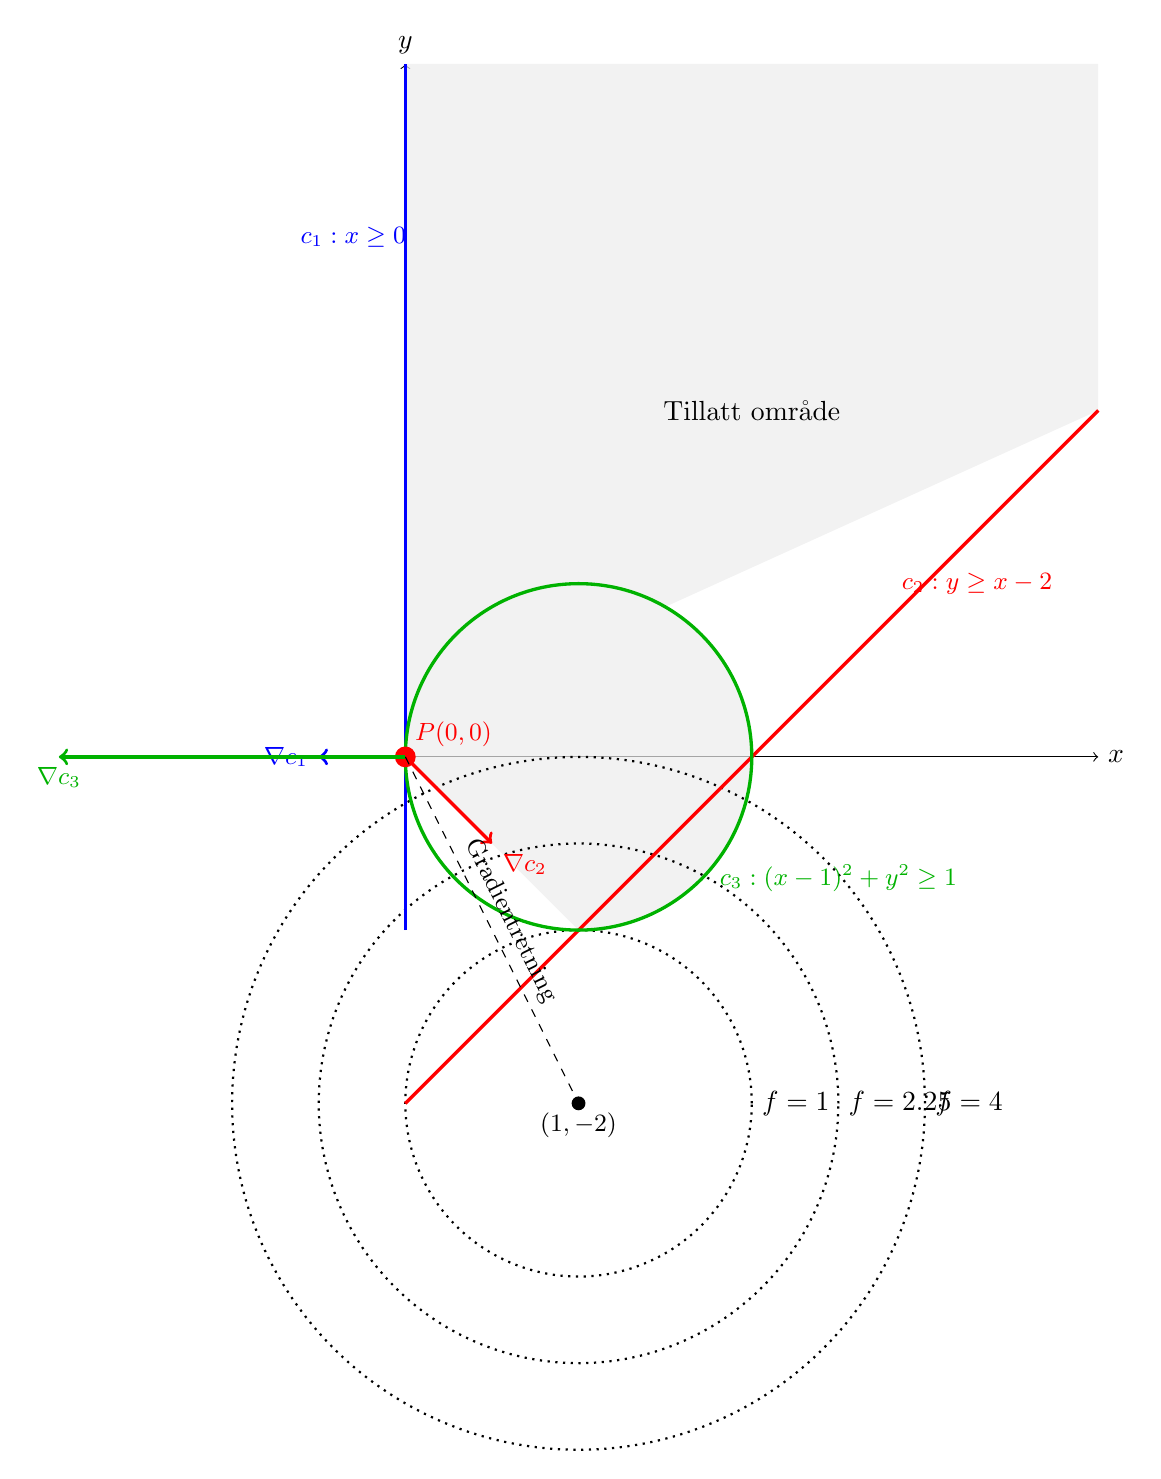
\begin{tikzpicture}[scale=2.2]
		% Koordinatsystem
		\draw[->] (-1,0) -- (4,0) node[right] {$x$};
		\draw[->] (0,-1) -- (0,4) node[above] {$y$};

		% Skravering av tillatt område først (under)
		\fill[gray!15, opacity=0.7] (0,0) -- (0,4) -- (4,4) -- (4,2) --
		plot[domain=60:0, smooth] ({1+cos(\x)},{sin(\x)}) --
		plot[domain=360:270, smooth] ({1+cos(\x)},{sin(\x)}) -- cycle;

		% Konturnivåer for målfunksjonen f(x,y) = (x-1)^2 + (y+2)^2
		\draw[black, dotted, thick] plot[domain=0:360,samples=100, smooth]
		({1+1.0*cos(\x)},{-2+1.0*sin(\x)}) node[right] {$f=1$};
		\draw[black, dotted, thick] plot[domain=0:360,samples=100, smooth]
		({1+1.5*cos(\x)},{-2+1.5*sin(\x)}) node[right] {$f=2.25$};
		\draw[black, dotted, thick] plot[domain=0:360,samples=100, smooth]
		({1+2.0*cos(\x)},{-2+2.0*sin(\x)}) node[right] {$f=4$};

		% Center point of objective function
		\fill[black] (1,-2) circle (0.04) node[below, font=\small] {$(1,-2)$};

		% x ≥ 0 (vertikal linje)
		\draw[blue, very thick] (0,-1) -- (0,4);

		% y ≥ x-2 (skrå linje)
		\draw[red, very thick] (0,-2) -- (4,2);

		% (x-1)^2 + y^2 ≥ 1 (sirkel med radius 1 sentrert i (1,0))
		\draw[green!70!black, very thick] (1,0) circle (1);

		% Forklarende tekst
		\node[blue, font=\small] at (-0.3,3) {$c_1: x \geq 0$};
		\node[red, font=\small] at (3.3,1) {$c_2: y \geq x-2$};
		\node[green!70!black, font=\small] at (2.5,-0.7) {$c_3: (x-1)^2 + y^2 \geq 1$};

		% Punkt der alle betingelser møtes (beregnet mer presist)
		\coordinate (P) at (0,0);
		\fill[red] (P) circle (0.06) node[above right, font=\small] {$P(0,0)$};

		% Gradienter ved punkt P
		\draw[->, very thick, blue] (P) -- +(-0.5,0) node[left, font=\small] {$\nabla c_1$};
		\draw[->, very thick, red] (P) -- +(0.5,-0.5) node[below right, font=\small] {$\nabla c_2$};
		\draw[->, very thick, green!70!black] (P) -- +(-2,0) node[below, font=\small] {$\nabla c_3$};

		% Feasible region label
		\node at (2,2) {Tillatt område};

		% Stiplet linje til optimal løsning
		\draw[black, dashed, ->] (P) -- (1,-2) node[midway, above, font=\small, sloped] {Gradientretning};
	\end{tikzpicture}
\end{center}

Ved punkt P hvor alle tre betingelser møtes, kan vi se at gradientene peker i forskjellige retninger og er lineært uavhengige. Derfor er LICQ oppfylt ved dette punktet. Dette er viktig for å kunne bruke KKT-betingelsene til å finne den optimale løsningen.
\subsection{Videre Merknader}

\begin{itemize}
	\item \textbf{Likhets- vs.\ ulikhetsbetingelser:} Likhetsbetingelsene \(c_i(x)=0\) er alltid aktive, mens en ulikhet \(c_j(x)\le 0\) kun er aktiv når \(c_j(x^*)=0\).
	\item \textbf{Jacobi-matrise:} Samler man gradientene som rader i en matrise, sier LICQ at denne matrisen har full rang, dvs. at antall aktive betingelser ikke overstiger \(\dim(x)\) og er lineært uavhengige.
	\item \textbf{Andre CQs:} Dersom LICQ ikke er oppfylt, kan man benytte andre såkalte \emph{constraint qualifications}, f.eks.\ Mangasarian--Fromovitz eller Slater-betingelser (for konvekse problemer), men da kan ikke entydigheten av multiplikatorer garanteres.
\end{itemize}

\subsection{Oppsummering}

Lineær Uavhengighetsbetingelse (LICQ) er en kjernenødvendighet for mange algoritmer og analytiske metoder innen ikke-lineær optimering. Den sikrer at de aktive betingelsene ved et punkt \(x^*\) er ``pent'' ordnet, i den forstand at ingen av gradientene er lineært avhengige. Når LICQ er gyldig, kan man utlede KKT-betingelsene og ofte fastslå entydige multiplikatorer. Som eksempel viser vi at betingelser som er multiple av hverandre (redundante) fører til brudd på LICQ og kan komplisere både teori og numeriske metoder.

\chapter{Optimalitetsbetingelser}

\section{Lagrangian-funksjonen}
\begin{definition}{The Lagrangian of a problem}{lagrangian}
	The Lagrangian of a problem is the function \(\mathcal{L}: \mathbb{R}^d \times \mathbb{R}^m \times \mathbb{R}^l \times \mathbb{R}^e \to \mathbb{R}\) defined as:
	\begin{align*}
		\mathcal{L}(x, \lambda, \mu, v) & = f(x) + \sum_{i\in \mathcal{I}} \lambda_i c_i(x) + \sum_{1 \leq i \leq m} \mu_i (Ax - b)_i + \sum_{1 \leq i \leq l} v_i (Cx - b)_i                               \\
		                                & = f(x) - \sum_{i \in \mathcal{I}} \lambda_i c_i(x) - \inner{\mu, Ax - b} - \inner{v, Cx - e}\footnote{\( (1) \iff \nabla_x \mathcal{L}(x, \lambda, \mu, v) = 0\)}
	\end{align*}
\end{definition}

Lagrangian-funksjonen gjør det mulig å håndtere betingelser ved å innføre multiplikatorer som vekter viktigheten av hver betingelse. Dette omformer et betinget optimeringsproblem til et ubetinget problem der vi søker sadelpunkter for Lagrangian-funksjonen.

\section{Farkas' lemma}

\begin{lemma}{Farka's Lemma}{farkas_lemma}
	Let \(A \in \mathbb{R}^{m \times n}\) and \(c \in \mathbb{R}^n\). Then, exactly one of the following statements is true:
	\begin{enumerate}
		\item[] \((1)\) There exists an \(x \in \mathbb{R}^n\) such that \(Ax \preceq 0\) and \(c^T x < 0\).
		\item[] \((2)\) There exists a \(y \in \mathbb{R}^m\) such that \(A^T y + c = 0\) and \(y \succeq 0\).
	\end{enumerate}
\end{lemma}

\begin{proof}
	\begin{enumerate}
		\item[] Assume that \((1)\) holds. Then \(Ax = b\) and \(x \ge 0\). If there exists a \(y\) such that \(y^T A \ge 0\), then
		      \[
			      y^T b = y^T Ax = (y^T A)x \ge 0,
		      \]
		      which contradicts \(y^T b < 0\).
		\item[] Assume that \((1)\) does not hold. We want to show that \((2)\) holds.

		      Let
		      \[
			      K = \{Ax \mid x \ge 0\}.
		      \]
		      Since \((1)\) does not hold, \(b \notin K\). Since \(K\) is a closed convex cone, by the separating hyperplane theorem, there exists a \(y \in \mathbb{R}^m\) such that
		      \[
			      y^T b < y^T z \quad \text{for all } z \in K.
		      \]
		      Since \(0 \in K\), we have \(y^T b < 0\).

		      Now, for any \(x \ge 0\), we have \(Ax \in K\), so \(y^T b < y^T Ax\).

		      Let \(x = e_i\), where \(e_i\) is the \(i\)-th standard basis vector. Then \(x \ge 0\), and
		      \[
			      y^T A e_i = (y^T A)_i > 0.
		      \]
		      Thus \(y^T A \ge 0\).
	\end{enumerate}

	\begin{center}
		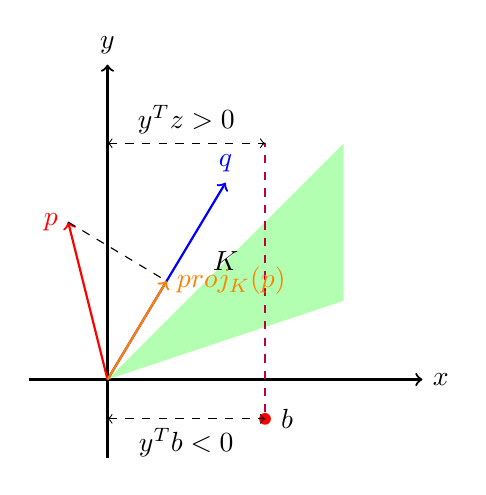
\begin{tikzpicture}
			\draw[->, thick] (-1, 0) -- (4, 0) node[right] {$x$};
			\draw[->, thick] (0, -1) -- (0, 4) node[above] {$y$};

			\fill[green!30] (0, 0) -- (3, 1) -- (3, 3) -- cycle;
			\node at (1.5, 1.5) {$K$};

			\node[circle, fill=red, inner sep=1.5pt, label=right:$b$] (b) at (2, -0.5) {};

			\draw[dashed, purple] (b) -- (2, 3);
			\draw[<->, dashed, black] (0, -0.5) -- (2, -0.5) node[midway, below, black] {$y^Tb < 0$};
			\draw[<->, dashed, black] (0, 3) -- (2, 3) node[midway, above, black] {$y^Tz > 0$};

			% Adding new vectors
			\draw[->, thick, blue] (0, 0) -- (1.5, 2.5) node[above] {$q$};
			\draw[->, thick, red] (0, 0) -- (-0.5, 2) node[left] {$p$};
			\draw[->, thick, orange] (0, 0) -- (0.75, 1.25) node[right] {$proj_K(p)$};
			\draw[dashed] (-0.5, 2) -- (0.75, 1.25);
		\end{tikzpicture}
	\end{center}

	The figure illustrates the geometric interpretation of Farkas' Lemma. The green region $K$ represents the cone of feasible points $\{Ax \mid x \ge 0\}$. The point $b$ (in red) lies outside this cone. The purple dashed line represents the separating hyperplane, which separates $b$ from $K$. Vector $p$ (in red) is projected onto the cone $K$, resulting in $proj_K(p)$ (in orange). Vector $q$ (in blue) lies inside the cone $K$. The black dashed lines show that the inner product $y^Tb$ is negative, while the inner product $y^Tz$ is positive for points $z$ in the cone $K$.
\end{proof}

\section[KKT-betingelser]{\gls{kkt-conditions}}

\begin{theorem}{KKT conditions}{kkt}
	\begin{align*}
		\mathcal{A}_1(x)            & := \{i \in \mathcal{I} \mid c_i(x) = 0\},                     \\
		\mathcal{A}_2(x)            & := \{1 \leq i \leq m \mid (Ax)_i = b_i\} \tag{Active indices} \\
		\text{Active indices at } x & \in \Omega                                                    \\
	\end{align*}

	\begin{itemize}
		\item \(A_i\) are the active constraints/indices at \(x\)
		\item \(C\) is the matrix of equality constraints.
		\item \(p\) is the direction of descent.
		\item \(x\) is the current point (feasible).
		\item \(T_{\Omega}(x)\) is the tangent cone at \(x\).
		\item \(c_i(x)\) is the value of the \(i\)-th constraint at \(x\).
		\item \(Ax\) is the value of the equality constraints at \(x\).
		\item \(b\) is the vector of equality constraints.
	\end{itemize}

	Assume that \emph{Slater's constraint} holds. Then, the following statements are equivalent:

	\begin{align*}
		p\in T_{\Omega}(x) & \Longleftrightarrow
		\begin{cases}
			\inner{\nabla c_i(x), p} \geq 0, & i \in \mathcal{A}_1(x) \\
			(Ax)_i \geq 0,                   & i \in \mathcal{A}_2(x) \\
			Cp = 0,                          &                        \\
		\end{cases}
	\end{align*}
\end{theorem}

\begin{theorem}{KKT conditions}{kkt_conditions}
	Assume \(c_i, i \in \mathcal{I}\) are concave in \(\mathcal{C}^1\),
	\(A\in \mathbb{R}^{m \times d}, b \in \mathbb{R}^m\) and \(C\in \mathbb{R}^{l \times d}\) and that \(f:\mathbb{R}^d \to \mathbb{R}\) is \(\mathcal{C}^1\). Assume that \emph{Slater's condition} holds.

	If \(x^\star\) is a local minimum of \(\min_x f(x)\) s.t.
	\[
		\begin{cases}
			c_i(x) \geq 0, & \forall i \in \mathcal{I} \\
			Ax \geq b,     &                           \\
			Cx = b,        &
		\end{cases}
	\]
	then there exists a \emph{Lagrange multipliers} \(\lambda^\star, \mu^\star\) with \(v \in \R^e\) s.t. the \emph{KKT conditions} hold:

	Then, the following statements are equivalent:
	\begin{align}
		\nabla f(x^\star) = \sum_{i\in \mathcal{I}} \lambda_i^\star \nabla c_i(x^\star) + A^T \mu^\star + C^T v^\star \\
		\begin{cases}
			c_i(x^\star) \geq 0, & \forall i \in \mathcal{I} \\
			Ax^\star \geq b,     &                           \\
			Cx^\star = e,        &                           \\
		\end{cases} \tag{Feasibility}                                                              \\
		\begin{cases}
			\lambda_i^\star \geq 0, & \forall i \in \mathcal{I} \\
			\mu_j^\star \in \geq 0, & \forall j \in \mathcal{J} \\
		\end{cases} \tag{Dual feasibility}                                                           \\
		\begin{cases}
			\lambda_i^\star c_i(x^\star) = 0, & \forall i \in \mathcal{I} \\
			\mu_j^\star C_j^T = 0,            & \forall j \in \mathcal{J} \\
		\end{cases} \tag{Complementary slackness}                                                 \\
		\begin{cases}
			\lambda_i^\star c_i(x^\star) = 0,      & \forall i \in \mathcal{I} \\
			\inner{\mu_j^\star, Ax^\star - b} = 0, & \forall j \in \mathcal{J} \\
		\end{cases} \tag{Complementary slackness}
	\end{align}
\end{theorem}

\begin{proof}{}{}
	We have the optimality condition:
	\[
		\inner{\nabla f(x^\star), p} \geq 0 \, \forall p \in T_{\Omega}(x^\star)
	\]
	\medskip
	\begin{align*}
		p \in T_{\Omega}(x^\star) \iff
		\begin{cases}
			\inner{\nabla c_i (x^\star), p }\geq 0                             & \forall i \in \mathcal{A}_1(x^\star) \\
			\text{or: there does not exist any } p \in \R^d \text{ such that:} &                                      \\
			\begin{cases}
				\inner{\nabla c_i (x^\star), p }\geq 0 & \forall i \in \mathcal{A}_1(x^\star) \\
				\inner{A_i^T , p }\geq 0               & \forall i \in \mathcal{A}_2(x^\star) \\
				\inner{ (C_i )^T, p } = 0              & \forall 1 \leq i \leq l              \\
				\inner{\nabla f (x^\star), p } < 0     &
			\end{cases}                             \\
			(Ap)_i \geq 0                                                      & \forall i \in \mathcal{A}_2(x^\star) \\
			Cp = 0                                                             &
		\end{cases}
	\end{align*}

	The second alternative is Farka's Lemma does not hold \(\implies\) The first holds.

	\begin{align*}
		\nabla f(x^\star) & = \sum_{i\in \mathcal{A}_1(x^\star)} \lambda_i^\star \nabla c_i(x^\star) + \sum_{i \in \mathcal{A}_2(x^\star)} \mu_i^\star A_i^T + \sum_{i=1}^l v_i^\star C_i^T \\
	\end{align*}

	For some  \(\lambda_i^\star \geq 0, \mu_i^\star \geq 0, v_i^\star \in \R\).

	Now define: \(\lambda_i^\star = 0 \) for \(i \notin \mathcal{A}_1(x^\star)\) and \(\mu_i^\star = 0\) for \(i \notin \mathcal{A}_2(x^\star)\).

	Then we have:
	\begin{align*}
		\nabla f(x^\star) & = \sum_{i\in \mathcal{I}} \lambda_i^\star \nabla c_i(x^\star) + \sum_{1 \leq i \leq m} \mu_i^\star A_i^T + \sum_{1 \leq i \leq l} v_i^\star C_i^T = \text{(1)} \\
	\end{align*}
	\qed
\end{proof}

\section{Geometrisk tolkning av KKT-betingelsene}

KKT-betingelsene har en klar geometrisk tolkning som er nyttig for å forstå deres betydning:

\begin{itemize}
	\item \textbf{Stasjonæritetsbetingelsen} (gradienten av Lagrangian er null) betyr at gradienten til målfunksjonen kan uttrykkes som en lineær kombinasjon av gradientene til de aktive betingelsene.
	\item \textbf{Primal feasibility} sikrer at løsningen tilfredsstiller alle opprinnelige betingelser.
	\item \textbf{Dual feasibility} (multiplikatorene for ulikheter er ikke-negative) sikrer at vi beveger oss i riktig retning langs betingelsene.
	\item \textbf{Komplementaritetsbetingelsen} forteller at en betingelse enten må være aktiv (likhet), eller så må den tilhørende multiplikatoren være null.
\end{itemize}

Denne geometriske tolkningen hjelper oss å visualisere hvordan KKT-betingelsene karakteriserer optimale punkter i et betinget optimeringsproblem.

\chapter{Konveks optimering}

\section{Egenskaper ved konvekse problemer}

Hvis et optimeringsproblem er konvekst, kan vi være sikre på at vi finner en global optimal løsning. Et konvekst optimeringsproblem har følgende egenskaper:
\begin{itemize}
	\item Målfunksjonen $f$ er konveks
	\item Likhetsbetingelsene $h_j$ er lineære (affine)
	\item Ulikhetsbetingelsene $g_i$ er konvekse
\end{itemize}

Konvekse optimeringsproblemer har flere fordelaktige egenskaper:
\begin{itemize}
	\item Ethvert lokalt minimum er også et globalt minimum
	\item KKT-betingelsene er både nødvendige og tilstrekkelige for optimalitet
	\item Det finnes effektive algoritmer for å løse konvekse problemer
\end{itemize}

\section{Dualitet i konveks optimering}

For konvekse optimeringsproblemer kan vi definere et dualt problem som gir en nedre grense på verdien av det primale problemet. Under visse betingelser, som Slaters betingelse, vil det primale og duale problemet ha samme optimale verdi - dette kalles "sterk dualitet".

Dualitetsteori gir oss viktige innsikter om optimale løsninger og multiplikatorer, og danner grunnlaget for mange effektive algoritmer for konveks optimering.